\chapter{Implementation}
The solution proposed in Chapters \ref{CHAPTER_proposed_algorithm} and \ref{CHAPTER_combination_with_existings_methods_of_inference}, except the verification of types, was implemented using the jInfer framework \cite{jinfer}. It is a framework for implementing methods of XML schema inference created as a software project at Faculty of Mathematics and Physics, Charles University in Prague. It is written in Java as a plugin for NetBeans platform.

The framework consists of modules representing logical parts of a process of inference. The main idea behind the modules is that they can be replaced by other modules with the same interface but different implementation and new modules can be connected to extend functionality.

\section{jInfer Process of Inference}
\begin{figure}
\label{FIG_jinfer_steps}
\caption{jInfer process of inference.}
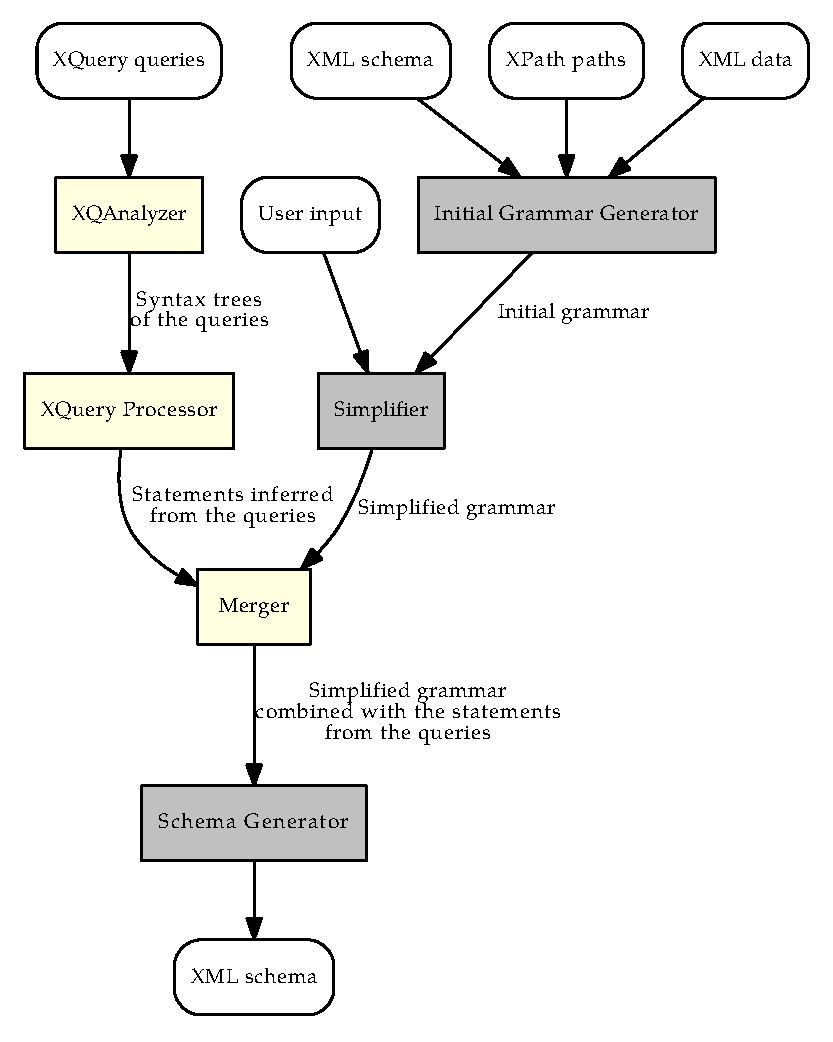
\includegraphics[scale=0.9]{jinfer_steps.eps}
\end{figure}

Figure \ref{FIG_jinfer_steps} shows the process of inference in jInfer. The grey and yellow rectangles represent steps of the inference, the white boxes represent input and output. Originally, the inference was composed of \textbf{Initial Grammar Generator}, \textbf{Simplifier}, and \textbf{Schema Generator} steps (grey). Steps (yellow) \textbf{XQAnalyzer}, \textbf{XQuery Processor}, and \textbf{Merger} are implementations of main parts of our proposed solution.

\begin{itemize}
\item \textbf{XQAnalyzer} - An implementation of the lexical and syntax analyses proposed in \cite{thesis_schejbal} and modified to create syntax trees. It parses input XQuery files and outputs their syntax trees.
\item \textbf{XQuery Processor} - An implementation of algorithms proposed in Chapter \ref{CHAPTER_proposed_algorithm}. In particular, construction of a syntax tree, static analysis of expression types, inference of built-in types, and key discovery. On input, it takes the syntax trees, and its output are statements inferred from the syntax tress. 
\item \textbf{Merger} - A step of inference responsible for combining the simplified grammar with the statements inferred by \textbf{XQuery Processor} as described in Chapter \ref{CHAPTER_combination_with_existings_methods_of_inference}, except the verification of types. Its result is the simplified grammar extended by the statements from \textbf{XQuery Processor} in a way that each statement is analysed and its information is assigned to concerned elements and attributes from the grammar. 
\end{itemize}

\section{jInfer Modules}
\begin{figure}
\label{FIG_jinfer_modules}
\caption{jInfer modules.}
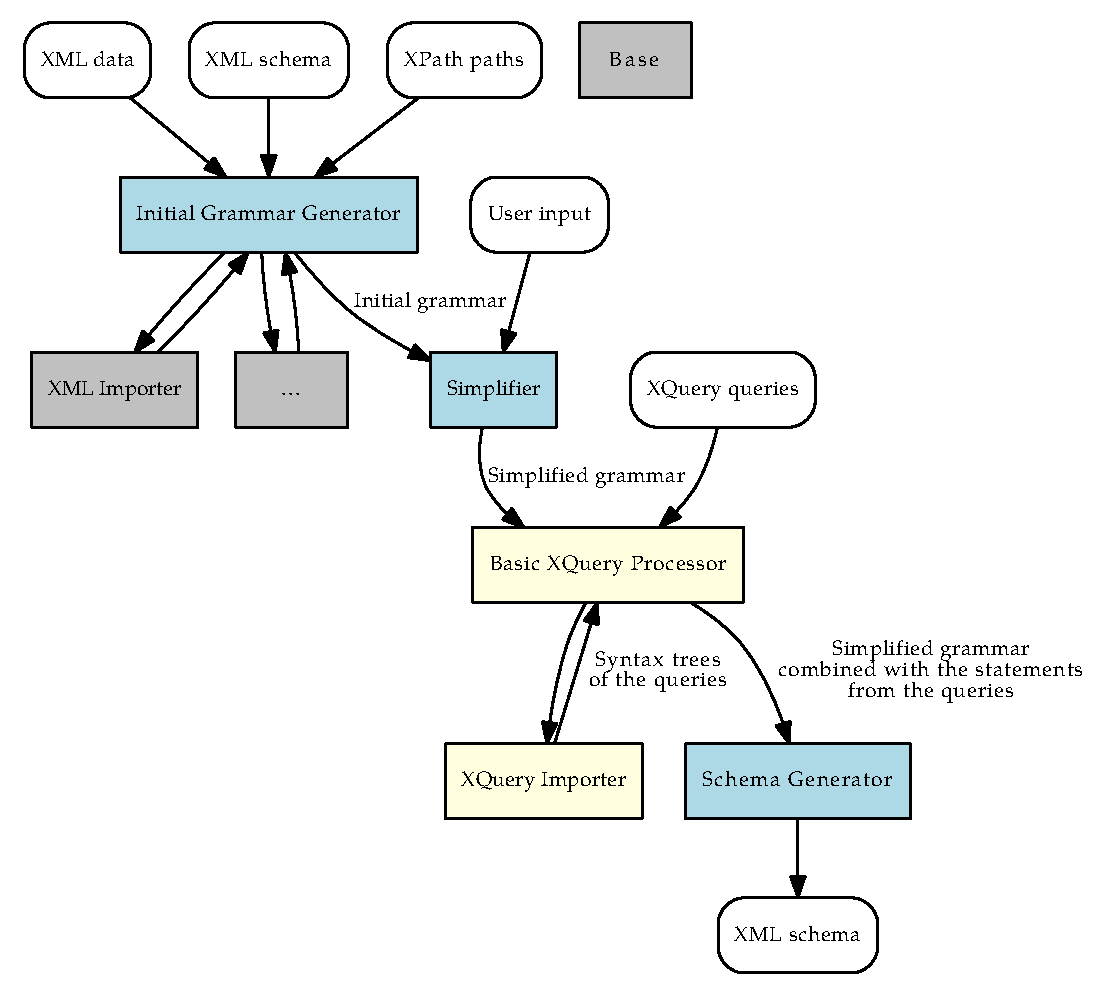
\includegraphics[scale=0.8]{jinfer_modules.eps}
\end{figure}

The previous section describes a high level schematic view of the process of inference. But, from a more technical view, jInfer modules do not utterly correspond with the steps of the presented process of inference.

The first difference is that none of the modules runs in parallel (in several threads) with other, as it is schematically shown in Figure \ref{FIG_jinfer_steps}. The modules run in a serial order as shown in Figure \ref{FIG_jinfer_modules}. The second difference is that one step is not always represented by one module, or one module is not always representing just one step.

Actually, the blue modules shown in \ref{FIG_jinfer_modules} are module abstractions with specified interface. Actual modules are then implementations complying the interface. Since we provide only one implementation of modules for the proposed solution, this is not very important for this work and we do not describe the principle in detail.

As in the previous section, newly added modules are those shown in yellow boxes. They are \textbf{XQuery Processor} and \textbf{XQuery Importer}. We also modified modules \textbf{Basic XSD Exporter} (an implementation of \textbf{Schema Generator} interface) and \textbf{Base} to extend their functionality.

\begin{itemize}
\item \textbf{Base} - This is module containing common classes used by other modules and defining interfaces. We added five packages to this module. Package \texttt{cz.cuni.mff.ksi.jinfer.base.objects.xquery.syntaxtree.nodes} implements the structure of syntax trees. Package \texttt{cz.cuni.mff.ksi.jinfer\-.base.interfaces.xquery} contains \texttt{Type} interface which is an interface for types used in the type analysis of syntax trees. Package \texttt{cz.cuni.mff.ksi\-.jinfer.base\-.objects.xquery.types} contains implementations of \texttt{Type} interface and type utility classes. Package \texttt{cz.cuni.mff.ksi.jinfer\-.base\-.objects.xquery.keys} provides representations of keys and foreign keys, and package \texttt{cz.cuni.mff.ksi\-.jinfer.base.objects.xsd} provides representation of XSD built-in atomic types.
\item \textbf{XQuery Importer} - This module represents \textbf{XQAnalyzer} step in Figure \ref{FIG_jinfer_steps}. It is responsible for creating syntax trees from input XQuery files (step 1).
\item \textbf{XQuery Processor} - The main module consisting of steps \textbf{XQuery Processor} and \textbf{Merger} in Figure \ref{FIG_jinfer_steps}. Package \texttt{cz.cuni.mff.ksi.jinfer\-.xqueryanalyzer} contains the main module class \texttt{XQueryAnalyzerImpl}. Other packages are \texttt{cz.cuni.mff.ksi.jinfer.xqueryanalyzer.-\\expressiontypesanalysis} implementing the static analysis of expression types (step 2), \texttt{cz.cuni.mff.ksi.jinfer.xqueryanalyzer.builtintype\-inference} implementing the inference of XSD built-in types (step 3), \texttt{cz\-.cuni.mff\-.ksi.jinfer\-.xqueryanalyzer.keydiscovery} and their subpackages implementing the key discovery (step 4), \texttt{cz.cuni.mff.ksi.jinfer\-.xqueryanalyzer.merger} implementing the merging with the grammar, and \texttt{cz.cuni.mff.ksi.jinfer.xqueryanalyzer.utils} containing various utilities.
\item \textbf{Basic XSD Exporter} - This is the module responsible for generating the resulting schema in XSD. It was modified to process the additional information assigned to the grammar in \textbf{XQuery Processor} module.
\end{itemize}